% Introdução

\documentclass[_ArquivoPrincipal.tex]{subfiles}

\begin{document}

%==================================================================================================
\section{Modelos de Turbulência} \label{MdT}
%==================================================================================================

A presente seção apresentará a fundamentação teórica dos modelos de turbulência baseado em grandes vórtices (LES) no item \ref{LES}, métodos variacionais multiescala (VMS) no item \ref{VMS} e \textit{Reynolds-Averaged Navier-Stokes} (RANS) no item \ref{RANS}.

%==================================================================================================
\subsection{\textit{Large Eddy Simulation}} \label{LES}
%==================================================================================================

A simulação de grandes vórtices se baseia na observação de que vórtices formados em pequenas escalas possuem comportamento isotrópico, o que permite uma modelagem dessas escalas, enquanto as grandes escalas podem ser computadas diretamente. Assim, realiza-se uma separação de escalas por meio de um filtro, que irá reescrever as equações de Navier-Stokes em termos de parcelas filtradas (ou de grandes escalas), denotadas para uma propriedade qualquer como $\bar{\phi}$, e uma parcela não filtrada (ou de escalas finas ou flutuações), denotada como $\phi'$ \cite{germano1991dynamic,hughes2000large}. Para isso, considera-se uma filtragem dada por:

\begin{equation}
    \bar{\phi}=\int_{\Dfil}{g(\BB{y},\yfil)\phi(\yfil,t)d\yfil}\text{,}
\end{equation}

\noindent em que $\Dfil$ é um subconjunto de $\Omega$ que determina a abrangência do filtro, $\yfil$ é um ponto na vizinhança de $\BB{y}$ e $g$ é o filtro, que deve possuir a propriedade de homogeneidade, $g(\BB{y},\yfil)=g(\BB{y}-\yfil)$.

\citeonline{hughes2000large} apresentam ainda uma possibilidade de abrangência de filtro dada por:

\begin{equation}
    \Dfil=\left\{\yfil\in\mathbb{R}^{n_{sd}}|\rho(\BB{y},\yfil)<\Delta/2\right\}\text{,}
\end{equation}

\noindent na qual $\Delta/2$ é o raio de abrangência do filtro centrado em $\BB{y}$ e $\rho$ é a distância Euclidiana de $\yfil$ à $\BB{y}$. A Figura \ref{fig:Filtro} apresenta esquematicamente o filtro considerado, assim como seu domínio de abrangência.

\begin{figure}[h]
    \centering
    \caption{Desenho esquemático do filtro considerado.}
    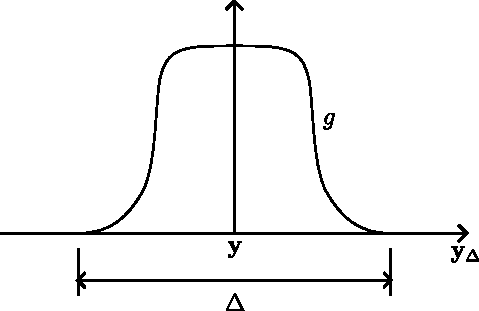
\includegraphics[width=0.5\linewidth]{Figuras/filtro.pdf}
    \\Fonte: \citeonline{hughes2000large} - Adaptado.
    \label{fig:Filtro}
\end{figure}

Dessa maneira, é possível separar os efeitos das grandes escalas e das pequenas escalas, o que pode ser observado esquematicamente na Figura \ref{fig:EfeitoFiltragem}, a qual apresenta o efeito da filtragem sobre um campo de velocidades $\BB{u}$.

\begin{figure}[h]
    \centering
    \caption{Efeito da filtragem sobre um campo de velocidades $\BB{u}$.}
    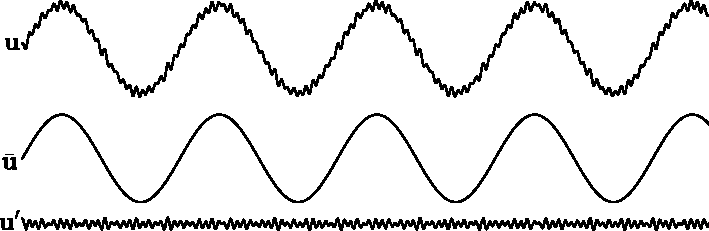
\includegraphics[width=.75\linewidth]{Figuras/efeito_filtragem.pdf}
    \\Fonte: \citeonline{hughes2000large} - Adaptado.
    \label{fig:EfeitoFiltragem}
\end{figure}

\textcolor{red}{Depois pesquisar sobre o problema do domínio $\Omega/\Omega_\Delta$}

Assim, em uma descrição Euleriana, pode-se obter as equações de Navier-Stokes filtradas:

\begin{equation}
    \left\{
   \begin{array}{ll}
        \rho\left(\apder{\BBB{u}}{t}+\NN\overline{(\BB{u}\otimes\BB{u})}-\BBB{f}\right)-\NN\cdot\overline{\tens}^T=\BB{0}&\text{ em }\Omega\text{,}\\
        \NN\cdot\BBB{u}=0&\text{ em }\Omega\text{.}
    \end{array}
    \right.
\end{equation}

\textcolor{red}{As condições de contorno são as mesmas, considerando c.c. filtradas?}

Pode-se perceber que o termo convectivo impede a completa separação dos termos $\BBB{u}$ e $\BB{u}'$ devido à sua natureza altamente não-linear. Por conta disso a parcela não filtrada não pode ser ignorada nesse problema, sendo necessário realizar algumas manipulações algébricas. Logo, sabendo-se que $\BB{u}=\BBB{u}+\BB{u}'$, pode-se reescrever a equação da conservação de movimento como:

\begin{equation}
    \rho\bigpar{\apder{\BBB{u}}{t}+\NN\overline{((\BBB{u}+\BB{u}')\otimes(\BBB{u}+\BB{u}'))}-\BBB{f}}-\NN\cdot\overline{\tens}^T=\BB{0}
\end{equation}

Nesse sentido, surgirão termos cruzados entre $\BBB{u}$ e $\BB{u}'$, o que serão condensados em um tensor de subescala (\textit{Subgrid-Scale} - SGS) $\BB{T}$ dado por \cite{piomelli1999large,hughes2000large}:

\begin{equation}
    \BB{T}=\BBB{u}\otimes\BBB{u}-\overline{\BB{u}\otimes\BB{u}}=-\bigpar{\BB{L}+\BB{C}+\BB{R}}\text{,}
\end{equation}

\noindent no qual $L_{ij}=\overline{\bar{u}_i\bar{u}_j}-\bar{u}_i\bar{u}_j$ é o tensor de Leonard, que representa as interações entre as grandes escalas, podendo ser determinado explicitamente utilizado para análise de erros, $C_{ij}=\overline{\bar{u}_iu'_j}+\overline{u'_i\bar{u}_j}$ é o tensor de termos cruzados, representando a interação entre as grandes e pequenas escalas e $R_{ij}=\overline{u'_iu'_j}$ é o tensor de tensões SGS de Reynolds, que rerepsenta a interação entre as pequenas escalas \cite{piomelli1999large}. Assim pode-se escrever que:

\begin{equation}
    \rho\bigpar{\apder{\BBB{u}}{t}+\NN\cdot(\BBB{u}\otimes\BBB{u})-\NN\cdot\BB{T}-\BBB{f}}-\NN\cdot\overline{\tens}^T=\BB{0}\text{.}
\end{equation}

Aplicando a incompressibilidade e substituindo-se $\tens$ pelo modelo constitutivo \ref{eq:ModConst}, sabendo que se trata de um tensor simétrico, tem-se que:

\begin{equation}
    \rho\bigpar{\apder{\BBB{u}}{t}+\BBB{u}\cdot\NN\BBB{u}-\NN\cdot\BB{T}-\BBB{f}}-2\mu\NN\cdot\deffil+\NN \bar{p}=\BB{0}\text{,}\label{eq:ConMasLES}
\end{equation}

\noindent sendo $\deffil=(\NN\BBB{u}+\NN^T\BBB{u})/2$. Assim, dividindo-se a Equação \ref{eq:ConMasLES} por $\rho$, substituindo $\deffil$ por \ref{eq:deftax1} e fazendo algumas manipulações tem-se que:

\begin{equation}
    \apder{\BBB{u}}{t}+\BBB{u}\cdot\NN\BBB{u}+\frac{\NN \bar{p}}{\rho}=\nu\Lapl\BBB{u}+\NN\cdot\BB{T}+\BBB{f}\text{,}
\end{equation}

\noindent em que $\Lapl\BBB{u}$ é o Laplaciano de $\BBB{u}$ e $\nu$ é a viscosidade dinâmica, dada por $\nu=\mu/\rho$.

Portanto, o problema se ser resolvido será:

\begin{equation}
    \left\{
   \begin{array}{ll}
        \apder{\BBB{u}}{t}+\BBB{u}\cdot\NN\BBB{u}+\frac{\NN \bar{p}}{\rho}=\nu\Lapl\BBB{u}+\NN\cdot\BB{T}+\BBB{f}&\text{ em }\Omega\text{,}\\
        \NN\cdot\BBB{u}=0&\text{ em }\Omega\text{,}
    \end{array}
    \right.
\end{equation}

\noindent o que revela a necessidade de se determinar um tensor $\BB{T}$, em especial o seu tensor desviador:

\begin{equation}
    \dev{\BB{T}}=\BB{T}-\frac{1}{3}\BB{I}\tr{\BB{T}}\text{,}
\end{equation}

\noindent que descreva adequadamente as interações entre diferentes escalas. Isso pode se tornar problemático uma vez que não se possui solução para as pequenas escalas. Dessa forma, considera-se um modelo capaz de fazer essa descrição, sendo observado, por exemplo, o modelo de viscosidade de vórtice de Smagorinsky, desenvolvido por \citeonline{smagorinsky1963general}. Nesse cenário faz-se que:

\begin{equation}
    \BB{T}_S=2\nu_T\deffil\text{,}
\end{equation}

\noindent sendo $\nu_T$ a viscosidade de vórtice SGS, dada por \cite{germano1991dynamic,piomelli1999large,hughes2000large}:

\begin{equation}
    \nu_T=(C_S\Delta)^2\norm{\deffil}\text{,}
\end{equation}

\noindent em que $C_S$ é a constante de Smagorinsky e $\norm{\deffil}$ é a magnitude do tensor de taxa de deformação em grandes escalas, dada por:

\begin{equation}
    \norm{\deffil}=(2\deffil\cdot\deffil)^{1/2}\text{.}
\end{equation}

Note que o tensor $\BB{T}_S$ é um tensor desviador, ou seja, $\BB{T}_S=\dev{\BB{T}_S}$.

\citeonline{germano1991dynamic,hughes2000large} ainda fazem algumas constatações sobre o modelo de Smagorinsky, os quais destacam-se o fato de $\BB{T}_S$ não possuir um comportamento assintótico próximo às paredes, o que se esperaria de $\BB{T}$, os valores de $C_S$ na presença de cisalhamento médio causaram amortecimentos excessivos e o tensor $\BB{T}_S$ impede a energia de fluir entre diferentes escalas, podendo ser significante em alguns casos.

Como tentativa de se resolver esses problemas, \citeonline{germano1991dynamic} propuseram assumir $C_S$ como uma função $C_S=C_S(\BB{y},t)$, premitindo, assim, que esse parâmetro se adapte para melhor modelar as pequenas escalas.

Com isso, e considerando que a dissipação de energia cinática é igual àquela produzida, pode-se obter a amplitude espectral da energia cinética ($E(k)$) como \cite{hughes2000large}:

\begin{equation}
    E(k)=\alpha\varepsilon^{2/3}k^{-5/3}\text{,}\label{eq:Ek1}
\end{equation}

\noindent em que $\alpha$ é a constante de Kolmogoroff, $\varepsilon$ é a dissipação turbulenta.

\textcolor{red}{descrever melhor o que é $k$, segundo \citeonline{hughes2000large}: $E(k)$ é a amplitude espectral da energia cinética, definida como a integral sobre a superfície de esferas parametrizadas com raio $k$ (?)}

Assim pode-se determinar o valor de $\norm{\deffil}$ como:

\begin{equation}
    \frac{1}{2}\norm{\deffil}=\int_0^{\bar{k}}{k^2E(k)dk}\text{,}\label{eq:ndeffil1}
\end{equation}

\noindent no qual $\bar{k}$ é o limite de resolução.

Substituindo \ref{eq:Ek1} em \ref{eq:ndeffil1}, resolvendo a integral e fazendo algumas manipulações algébricas, tem-se que:

\begin{equation}
    \norm{\deffil}^3=\bigpar{\frac{3\alpha}{2}}^{3/2}\bar{k}^2\varepsilon\text{.}
\end{equation}

Dessa forma, realiza-se o balanço da energia cinética turbulenta dissipada com a produzida, obtendo-se:

\begin{equation}
    \varepsilon=\BB{T}_S\cdot\deffil\text{,}
\end{equation}

\noindent que, após seu desenvolvimento, tem-se uma expressão que relaciona os valores de $C_S$, $\Delta$ e $\nu_T$ com $\bar{k}$:

\begin{equation}
    C_S\Delta=\bigpar{\frac{2}{3\alpha}}^{3/4}\bar{k}^{-1}\text{ e}
\end{equation}

\begin{equation}
    \nu_T=\bigpar{\frac{2}{3\alpha}}\varepsilon^{1/3}\bar{k}^{-4/3}\text{.}
\end{equation}

%==================================================================================================
\subsection{\textit{Variational Multiscale Methods}} \label{VMS}
%==================================================================================================

O Método Variacional Multiescala foi introduzido por \citeonline{hughes1995multiscale,hughes1998variational,hughes2000large}, o qual faz a separação dos espaços de tentativas e de testes em subespaços que representem as escalas grosseiras, que se tratam de subespaços de dimensões finitas e denotadas por uma barra, e as escalas finas, que são subespaços de infinitas dimensões e denotadas por $'$, ou seja:

\begin{subequations}
    \begin{align}
        &\script{S}_u=\bar{\script{S}}_u\oplus\script{S}'_u\text{,}\\
        &\script{S}_p=\bar{\script{S}}_p\oplus\script{S}'_p\text{,}\\
        &\script{V}_u=\bar{\script{V}}_u\oplus\script{V}'_u\text{ e}\\
        &\script{V}_p=\bar{\script{V}}_p\oplus\script{V}'_p\text{.}
    \end{align}
\end{subequations}

Inicialmente será abordado uma técnica baseada em uma descrição Euleriana com domínio fixo, para maior familiarização com o método, e na sequência será apresentada uma formulação em descrição ALE utilizando domínio móvel.

O sistema a ser resolvido parte do apresentado em \ref{eq:NS-Euler}, que em sua forma fraca se encontra em \ref{eq:WeakForm2}. Primeiramente se a separação dos membros em:

\begin{subequations}
    \begin{align}
        &\BB{u}=\BBB{u}+\BB{u}'\text{,}\\
        &p=\bar{p}+p'\text{,}\\
        &\BB{w}=\BBB{w}+\BB{w}'\text{ e}\\
        &q=\bar{q}+q'\text{,}
    \end{align}
\end{subequations}

\noindent em que se adota $\BB{w}=\BBB{w}$ e $q=\bar{q}$ e as escalas finas $\BB{u}'$ e $p'$ podem ser modeladas como:

\begin{subequations}
    \begin{equation}
        \BB{u}'=-\frac{\tau_{\sups}}{\rho}\rM\text{ e}
    \end{equation}
    \begin{equation}
        p'=-\rho\nu_{\lsic}\rC\text{,}
    \end{equation}
\end{subequations}

\noindent nas quais $\tau_{\sups}$ e $\nu_{\lsic}$ são termos estabilizadores, dados por \cite{bazilevs2013computational}:
%página 80 do pdf de hughes2013 e 65 de fernandes2020

\begin{subequations}
    \begin{equation}
        \tau_{\sups}=\bigpar{\frac{4}{\Delta t^2}+\BBB{u}\cdot\BB{G}\BBB{u}+C_I\nu^2\BB{G}:\BB{G}}^{-1/2}\text{ e}
    \end{equation}
    \begin{equation}
        \nu_{\lsic}=(\tr{\BB{G}}\tau_{\sups})^{-1}\text{,}
    \end{equation}
    \label{eq:TermEstab}
\end{subequations}

\noindent onde $C_I$ é uma constante e:

\begin{equation}
    \BB{G}=\frac{\partial\BB{\xi}}{\partial\BB{x}}^T\frac{\partial\BB{\xi}}{\partial\BB{x}}\text{.}
\end{equation}

Já os termos $\rM$ e $\rC$ são os resíduos associados à equação de conservação da quantidade de movimento e da continuidade, respectivamente:

\begin{subequations}
    \begin{equation}
        \rM=\rho\bigpar{\der{\BBB{u}}{t}+\BBB{u}\cdot\NN\BBB{u}-\BBB{f}}-\NN\cdot\tens(\BBB{u},\bar{p})\text{ e}
    \end{equation}
    \begin{equation}
        \rC=\NN\cdot\BBB{u}\text{.}
    \end{equation}
\end{subequations}

Outra forma de se modelar os parâmetros estabilizadores pode ser dado por \cite{bazilevs2013computational}:

\begin{subequations}
    \begin{equation}
        \tau_{\sups}=\bigpar{\frac{1}{\tau_{\sugn 1}^2}+\frac{1}{\tau_{\sugn 2}^2}+\frac{1}{\tau_{\sugn 3}^2}}^{-1/2}\text{ e}
    \end{equation}
    \begin{equation}
        \nu_{\lsic}=\tau_{\sups}\norm{\BBB{u}}^2\text{,}
    \end{equation}
\end{subequations}

\noindent tal que:

\begin{subequations}
    \begin{align}
        &\tau_{\sugn 1}=\bigpar{\sum_{a=1}^{n_{en}}{\abs{\BBB{u}\cdot\NN N_a}}}^{-1}\text{,}\\
        &\tau_{\sugn 2}=\frac{\Delta t}{2}\text{,}\\
        &\tau_{\sugn 3}=\frac{h_{\rgn}^2}{4\nu}\text{,}\\
        &h_\rgn=2\bigpar{\sum_{a=1}^{n_{en}}{\abs{\BB{r}\cdot\NN N_a}}}^{-1}\text{ e}\\
        &\BB{r}=\frac{\NN\norm{\BBB{u}}}{\norm{\NN\norm{\BBB{u}}}}\text{.}
    \end{align}    
\end{subequations}

Assim, obtém-se o problema do Método Variacional Multiescala Baseado em Resíduos (\textit{Residual-Based Variational Multiscale} - RBVMS) que busca determinar $\BBB{u}\in\bar{\script{S}}_u$ e $\bar{p}\in\bar{\script{S}}_p$, tais que para todo $\BBB{w}\in\bar{\script{V}}_u$ e $\bar{q}\in\bar{\script{V}}_p$ \cite{bazilevs2013computational}:

\begin{equation}
\begin{split}
    &\int_\Omega{\BBB{w}\cdot\rho\bigpar{\der{\BBB{u}}{t}+\BBB{u}\cdot\NN\BBB{u}-\BBB{f}}d\Omega}+\int_\Omega{\BB{\varepsilon}(\BBB{w}):\tens(\BBB{u},\bar{p})d\Omega}-\\
    &\int_{\Gamma_N}{\BBB{w}\cdot\BBB{h}d\Gamma_N}+\int_\Omega{\bar{q}\NN\cdot\BBB{u}d\Omega}+\\
    &\sum_{e=1}^{n_{el}}{\int_{\Omega^e}{\tau_\sups\bigpar{\BBB{u}\cdot\NN\BBB{w}+\frac{\NN\bar{q}}{\rho}}\cdot\rM d\Omega^e}}+\\
    &\sum_{e=1}^{n_{el}}{\int_{\Omega^e}{\rho\nu_\lsic\NN\cdot\BBB{w}\rC d\Omega^e}}-\\
    &\sum_{e=1}^{n_{el}}{\int_{\Omega^e}{\tau_\sups\BBB{w}\cdot(\rM\cdot\NN\BBB{u})d\Omega^e}}-\\
    &\sum_{e=1}^{n_{el}}{\int_{\Omega^e}{
    \frac{\NN\BBB{w}}{\rho}:(\tau_\sups\rM)\otimes(\tau_\sups\rM)d\Omega^e}}=0
    \text{.}
    \label{eq:RBVMS1}
\end{split}
\end{equation}

Para a discretização do problema pode-se realizar a separação da dependência espacial e temporal para os espaços tentativas e testes como:

\begin{subequations}
    \begin{align}
        &\BBB{u}(\BB{y},t)=\sum_{\BB{\eta}^s}{\BB{u}_a(t)N_a(\BB{y})}\text{,}\\
        &\bar{p}(\BB{y},t)=\sum_{\BB{\eta}^s}{p_a(t)N_a(\BB{y})}\text{,}\\
        &\BBB{w}(\BB{y})=\sum_{\BB{\eta}^w}{\BB{w}_aN_a(\BB{y})}\text{ e}
        \label{eq:w-sep}\\
        &\bar{q}(\BB{y})=\sum_{\BB{\eta}^w}{q_aN_a(\BB{y})}\text{.}
        \label{eq:q-sep}
    \end{align}
\end{subequations}

Substituindo \ref{eq:w-sep} e \ref{eq:q-sep} em \ref{eq:RBVMS1} obtém-se dois vetores que representam o resíduo das equações da conservação da quantidade de movimento e da continuidade, nos quais $\BBB{w}_a$ e $q_a$ são arbitrários:

\begin{subequations}
    \begin{equation}
        \NM=[(N_\mathrm{M})_{a,i}]\text{,}
    \end{equation}
    \begin{equation}
        \NC=[(N_\mathrm{C})_a]\text{,}
    \end{equation}
    \begin{equation}
    \begin{split}
        (N_\mathrm{M})_{a,i}=&
        \int_{\Omega}{N_a\bhat{e}_i\cdot\rho\bigpar{\der{\BBB{u}}{t}+\BBB{u}\cdot\NN\BBB{u}-\BBB{f}}d\Omega}+\\
        &\int_{\Omega}{\Def(N_a\bhat{e}_i):\tens(\BBB{u},\bar{p})d\Omega}-\int_{\Gamma_N}{N_a\bhat{e}_i\cdot\BBB{h}d\Gamma_N}+\\
        &\sum_{e=1}^{n_{el}}{\int_{\Omega^e}{\tau_\sups(\BBB{u}\cdot\NN N_a\bhat{e}_i)\cdot\rM d\Omega^e}}+\\
        &\sum_{e=1}^{n_{el}}{\int_{\Omega^e}{\rho\nu_\lsic(\NN\cdot N_a\bhat{e}_i)\rC d\Omega^e}}-\\
        &\sum_{e=1}^{n_{el}}{\int_{\Omega^e}{\tau_\sups N_a\bhat{e}_i\cdot(\rM\cdot\NN\BBB{u}) d\Omega^e}}-\\
        &\sum_{e=1}^{n_{el}}{\int_{\Omega^e}{\frac{\NN N_a\bhat{e}_i}{\rho}:(\tau_\sups\rM)\otimes(\tau_\sups\rM) d\Omega^e}}
        \text{,}
    \end{split}
    \end{equation}
    \begin{equation}
        (N_\mathrm{C})_a=\int_{\Omega}{N_a\NN\cdot\BBB{u}d\Omega}+\sum_{e=1}^{n_{el}}{\int_{\Omega^e}{\tau_\sups\frac{\NN N_a}{\rho}\cdot\rM d\Omega^e}}
    \end{equation}
\end{subequations}

Sendo os vetores $\BB{U}=[\BB{u}_B]$, $\dot{\BB{U}}=[\dot{\BB{u}}_B]$ e $\BB{P}=[p_B]$, que representam, respectivamente, os graus de liberdade em velocidades, primeira derivada temporal das velocidades e pressões nodais, então o problema a ser resolvido será dado por: encontrar $\BB{U}$, $\dot{\BB{U}}$ e $\BB{P}$, tais que:

\begin{subequations}
    \begin{align}
        &\NM(\BB{U},\dot{\BB{U}},\BB{P})=\BB{0}\text{ e}\\
        &\NC(\BB{U},\dot{\BB{U}},\BB{P})=\BB{0}\text{.}        
    \end{align}
\end{subequations}

Uma formulação alternativa à apresentada é apresentada por \citeonline{bazilevs2013computational}, denominada como SUPG/PSPG, onde se omite os dois últimos termos da equação \ref{eq:RBVMS1} e se utiliza de valores diferentes de $\tau$ para as equações de conservação da quantidade de movimento e da continuidade, resultando em:

\begin{equation}
\begin{split}
    &\int_\Omega{\BBB{w}\cdot\rho\bigpar{\der{\BBB{u}}{t}+\BBB{u}\cdot\NN\BBB{u}-\BBB{f}}d\Omega}+\int_\Omega{\BB{\varepsilon}(\BBB{w}):\tens(\BBB{u},\bar{p})d\Omega}-\\
    &\int_{\Gamma_N}{\BBB{w}\cdot\BBB{h}d\Gamma_N}+\int_\Omega{\bar{q}\NN\cdot\BBB{u}d\Omega}+\\
    &\sum_{e=1}^{n_{el}}{\int_{\Omega^e}{\tau_\supg\bigpar{\BBB{u}\cdot\NN\BBB{w}}\cdot\rM d\Omega^e}}+\\
    &\sum_{e=1}^{n_{el}}{\int_{\Omega^e}{\tau_\pspg\bigpar{\frac{\NN\bar{q}}{\rho}}\cdot\rM d\Omega^e}}+\\
    &\sum_{e=1}^{n_{el}}{\int_{\Omega^e}{\rho\nu_\lsic\NN\cdot\BBB{w}\rC d\Omega^e}}=0
    \text{,}
    \label{eq:SUPG-PSPG}
\end{split}
\end{equation}

\noindent na qual, segundo os autores, adota-se $\tau_\pspg=\tau_\supg=\tau_\sups$ para uma boa variedade de problemas.

Por sua vez, a formulação baseada em uma descrição ALE parte das equações apresentadas em \ref{eq:NS-ALE}, cujo problema semi-discreto pode ser dado por:

\begin{equation}
\begin{split}
    &\int_\Omega{\BB{w}\cdot\rho\bigpar{\apderxh{\BB{u}}{t}+(\BB{u}-\uhat)\cdot\NN\BB{u}-\BB{f}}d\Omega}+\int_\Omega{\Def({\BB{w}}):\tens(\BB{u},p)d\Omega}-\\
    &\int_{\Gamma_N}{\BB{w}\cdot\BB{h}d\Gamma}+\int_\Omega{q\NN\cdot\BB{u}d\Omega}=0    
\end{split}
\end{equation}

Portanto o problema semi-discreto em formulação RBVMS de escoamentos incompressíveis segundo uma descrição ALE será: encontrar $\BBB{u}\in\bar{\script{S}}_u$ e $\bar{p}\in\bar{\script{S}}_p$, tais que para todo $\BBB{w}\in\bar{\script{V}}_u$ e $\bar{q}\in\bar{\script{V}}_p$ \cite{bazilevs2013computational}:

\begin{equation}
\begin{split}
    &\int_\Omega{\BBB{w}\cdot\rho\bigpar{\apderxh{\BBB{u}}{t}+(\BBB{u}-\uhat)\cdot\NN\BBB{u}-\BBB{f}}d\Omega}+\int_\Omega{\BB{\varepsilon}(\BBB{w}):\tens(\BBB{u},\bar{p})d\Omega}-\\
    &\int_{\Gamma_N}{\BBB{w}\cdot\BBB{h}d\Gamma_N}+\int_\Omega{\bar{q}\NN\cdot\BBB{u}d\Omega}+\\
    &\sum_{e=1}^{n_{el}}{\int_{\Omega^e}{\tau_\sups\bigpar{(\BBB{u}-\uhat)\cdot\NN\BBB{w}+\frac{\NN\bar{q}}{\rho}}\cdot\rM d\Omega^e}}+\\
    &\sum_{e=1}^{n_{el}}{\int_{\Omega^e}{\rho\nu_\lsic\NN\cdot\BBB{w}\rC d\Omega^e}}-\\
    &\sum_{e=1}^{n_{el}}{\int_{\Omega^e}{\tau_\sups\BBB{w}\cdot(\rM\cdot\NN\BBB{u})d\Omega^e}}-\\
    &\sum_{e=1}^{n_{el}}{\int_{\Omega^e}{
    \frac{\NN\BBB{w}}{\rho}:(\tau_\sups\rM)\otimes(\tau_\sups\rM)d\Omega^e}}=0
    \text{,}
    \label{eq:RBVMS-ALE}
\end{split}
\end{equation}

\noindent em que os termos estabilizadores $\tau_\sups$ e $\nu_\lsic$ são alterados das equações \ref{eq:TermEstab}, onde se considera, ao invés da velocidade do fluido $\BBB{u}$, a velocidade relativa à malha ($\BBB{u}-\uhat$), ou seja, $\BBB{u}\gets\BBB{u}-\uhat$.

Para o problema discretizado utiliza-se as seguintes expressões de aproximação dos espaços tentativas e testes:

\begin{subequations}
    \begin{align}
        &\BBB{u}(\BB{y},t)=\sum_{\BB{\eta}^s}{\BB{u}_a(t)N_a(\BB{y},t)}\text{,}\\
        &\bar{p}(\BB{y},t)=\sum_{\BB{\eta}^s}{p_a(t)N_a(\BB{y},t)}\text{,}\\
        &\BBB{w}(\BB{y})=\sum_{\BB{\eta}^w}{\BB{w}_aN_a(\BB{y},t)}\text{ e}\\
        &\bar{q}(\BB{y})=\sum_{\BB{\eta}^w}{q_aN_a(\BB{y},t)}\text{,}
    \end{align}
\end{subequations}

\noindent onde as funções de forma $N_a(\BB{y},t)$ são definidas como:

\begin{equation}
    N_a(\BB{y},t)=\hat{N}_a(\bhat{f}^{-1}(\BB{y},t))\text{,}
\end{equation}

\noindent em que $\bhat{f}(\BB{y},t)$ é a função de mudança de configuração de $\hat{\Omega}\to\Omega$, conforme apresentado no item \ref{CFD-ALE}, dada em sua forma discreta por:

\begin{equation}
    \bhat{f}(\bhat{x},t)=\sum_{a\in\BB{\eta}^s}{(\bhat{x}_a+\Delta\bhat{x}_a(t))\hat{N}_a(\bhat{x})}\text{,}
\end{equation}

\noindent sendo $\bhat{x}_a$ as posições nodais em $\hat{\Omega}$, $\Delta\bhat{x}(t)$ o deslocamento nodal e $\hat{N}_a$ é a função de forma fixa da discretização de $\hat{\Omega}$. Nota-se, portanto, que as funções $N_a(\BB{y},t)$ possuem dependência temporal devido à movimentação da malha.

Com isso, define-se os vetores de resíduos da conservação de quantidade de movimento de da continuidade como:

\begin{subequations}
    \begin{equation}
        \NM=[(N_\mathrm{M})_{a,i}]\text{,}
    \end{equation}
    \begin{equation}
        \NC=[(N_\mathrm{C})_a]\text{,}
    \end{equation}
    \begin{equation}
    \begin{split}
        (N_\mathrm{M})_{a,i}=&
        \int_{\Omega}{N_a\bhat{e}_i\cdot\rho\bigpar{\apderxh{\BBB{u}}{t}+(\BBB{u}-\uhat)\cdot\NN\BBB{u}-\BBB{f}}d\Omega}+\\
        &\int_{\Omega}{\Def(N_a\bhat{e}_i):\tens(\BBB{u},\bar{p})d\Omega}-\int_{\Gamma_N}{N_a\bhat{e}_i\cdot\BBB{h}d\Gamma_N}+\\
        &\sum_{e=1}^{n_{el}}{\int_{\Omega^e}{\tau_\sups((\BBB{u}-\uhat)\cdot\NN N_a\bhat{e}_i)\cdot\rM d\Omega^e}}+\\
        &\sum_{e=1}^{n_{el}}{\int_{\Omega^e}{\rho\nu_\lsic(\NN\cdot N_a\bhat{e}_i)\rC d\Omega^e}}-\\
        &\sum_{e=1}^{n_{el}}{\int_{\Omega^e}{\tau_\sups N_a\bhat{e}_i\cdot(\rM\cdot\NN\BBB{u}) d\Omega^e}}-\\
        &\sum_{e=1}^{n_{el}}{\int_{\Omega^e}{\frac{\NN N_a\bhat{e}_i}{\rho}:(\tau_\sups\rM)\otimes(\tau_\sups\rM) d\Omega^e}}
        \text{,}
    \end{split}
    \end{equation}
    \begin{equation}
        (N_\mathrm{C})_a=\int_{\Omega}{N_a\NN\cdot\BBB{u}d\Omega}+\sum_{e=1}^{n_{el}}{\int_{\Omega^e}{\tau_\sups\frac{\NN N_a}{\rho}\cdot\rM d\Omega^e}}
    \end{equation}
\end{subequations}

Assim, pretende-se determinar os vetores $\BB{U}$, $\dot{\BB{U}}$ e $\BB{P}$, tais que:

\begin{subequations}
    \begin{align}
        &\NM(\BB{U},\dot{\BB{U}},\BB{P})=\BB{0}\text{ e}\\
        &\NC(\BB{U},\dot{\BB{U}},\BB{P})=\BB{0}\text{.}        
    \end{align}
\end{subequations}

\textcolor{red}{Continuar escrevendo sobre ALE (?)}

%==================================================================================================
\subsection{\textit{Reynolds-Averaged Navier-Stokes}} \label{RANS}
%==================================================================================================

Na tentativa de se obter soluções aproximativas para as equações de Navier-Stokes, são desenvolvidas técnicas de aproximação, baseadas em equações diferenciais. Uma dessas aproximações, denominada de \textit{Reynolds-Averaged Navier-Stokes} (RANS) busca encontrar uma solução a partir da decomposição de Reynolds. Nesse contexto, observa-se que simulações feitas utilizando RANS são mais eficientes computacionalmente que aquelas feitas a partir de LES, além de possuírem uma implementação mais facilitada \cite{alfonsi2009reynolds, ling2015evaluation}. Ainda segundo \citeonline{alfonsi2009reynolds}, problemas envolvendo RANS podem ser classificados dependendo da quantidade de equações diferenciais resolvidas, em que cada equação adicionada refere-se ao transporte de uma propriedade relativa à turbulência.

Em uma descrição Euleriana, sua obtenção parte da equação \ref{eq:NS-Euler} e considera-se que uma propriedade $\phi$ pode ser decomposta em duas parcelas: uma referente à média temporal, denotada por uma barra ($\bar{\phi}(\BB{y})$), dada por \cite{tennekes1972first,speziale1991analytical}:

\begin{equation}
    \bar{\phi}(\BB{y})=\lim_{T\to\infty}{\frac{1}{T}\int_{t_0}^{t_0+T}{\phi(\BB{y},t)dt}}\text{,}
\end{equation}

\noindent e uma referente à flutuações no espaço-tempo, denotada por $\phi'(\BB{y},t)$, ou seja, $\phi(\BB{y},t)=\bar{\phi}(\BB{y})+\phi'(\BB{y},t)$.

Vale ressaltar algumas propriedades interessantes relacionadas à média de uma propriedade ($\phi$, $\phi_1$ ou $\phi_2$ quaisquer), tais como:

\begin{enumerate}[label=\alph*.]
    \item $\bar{\phi'}(\BB{y})=0$;
    \item $\bar{\bar{\phi}}=\bar{\phi}$;
    \item $\bar{\phi_1+\phi_2}=\bar{\phi}_1+\bar{\phi}_2$;
    \item $\bar{\phi_1\bar{\phi}_2}=\bar{\phi}_1\bar{\phi}_2$;
    \item $\bar{\phi_1\phi_2}=\bar{\phi}_1\bar{\phi}_2+\bar{\phi_1'\phi_2'}$; e
    \item $\bar{\der{\phi}{y_i}}=\der{\bar{\phi}}{y_i}$.
\end{enumerate}

Assim, pode-se tomar a média das Equações de Navier-Stokes, obtendo-se:

\begin{equation}
    \left\{
   \begin{array}{ll}
        \rho\bigpar{\bar{\apder{\BB{u}}{t}}+\bar{\BB{u}\cdot\NN\BB{u}}-\bar{\BB{f}}}-\bar{\NN\cdot\tens^T}=\BB{0}&\text{ em }\Omega\text{,}\\
        \bar{\NN\cdot\BB{u}}=0&\text{ em }\Omega\text{.}
    \end{array}
    \right.
\end{equation}

Note que, ao tomar a média temporal, o problema se torna independente do tempo. Portanto o termo referente à derivada temporal de $\BB{u}$ desaparece. Assim, aplicando também o modelo constitutivo apresentado em \ref{MC}, o problema se torna:

\begin{equation}
    \left\{
   \begin{array}{ll}
        \rho\bigpar{\bar{\BB{u}\cdot\NN\BB{u}}-\bar{\BB{f}}}-\NN\cdot\bar{(2\mu\deftax)}+\NN\bar{p}=\BB{0}&\text{ em }\Omega\text{,}\\
        \NN\cdot\bar{\BB{u}}=0&\text{ em }\Omega\text{.}
    \end{array}
    \right.
\end{equation}

Realizando a separação dos parâmetros em suas respectivas parcelas na equação da conservação de movimento, tem-se que:

\begin{equation}
    \rho\bigpar{\bar{(\bar{\BB{u}}+\BB{u}')\cdot\NN(\bar{\BB{u}}+\BB{u}')}-\bar{\BB{f}}}-
    \mu\NN\cdot(\bar{\NN(\bar{\BB{u}}+\BB{u}')+\NN^T(\bar{\BB{u}}+\BB{u}')})+\NN\bar{p}=\BB{0}\text{,}   
\end{equation}

\noindent que leva à seguinte expressão simplificada:

\begin{subequations}
\begin{equation}
        \rho\bigpar{\bar{\BB{u}}\cdot\NN\bar{\BB{u}}+\NN\cdot\bar{(\BB{u}'\otimes\BB{u}')}-\bar{\BB{f}}}-
        \mu\Lapl{\BB{u}}+\NN\bar{p}=\BB{0}\text{, ou}
\end{equation}
\begin{equation}
        \rho\bigpar{\bar{u}_i\der{\bar{u}_j}{y_i}+\der{\bar{u_i'u_j'}}{y_i}-\bar{f}_j}-\mu\frac{\partial^2\bar{u}_j}{\partial y_i\partial y_i}+\der{\bar{p}}{y_j}=0\text{,}
\end{equation}
\label{eq:RANS-estac}
\end{subequations}

\noindent a qual representa a equação de Navier-Stokes para escoamentos incompressíveis em regime estacionário em uma formulação RANS \cite{chou1945velocity,alfonsi2009reynolds}.

Além disso, é possível fazer a substituição de $\BB{u}=\umed+\BB{u}'$ e $p=\bar{p}+p'$ na equação da quantidade de movimento, o que leva a:

\begin{equation}
\begin{split}
    &\rho\bigpar{\apder{\ufl}{t}+\umed\cdot\NN\umed+\umed\cdot\NN\ufl+\ufl\cdot\NN\umed+\ufl\cdot\NN\ufl-\bar{\BB{f}}}-\\
    &\mu\Lapl\umed-\mu\Lapl\ufl+\NN\bar{p}+\NN p'=\BB{0}\text{.}
\end{split}
\label{eq:NS-RANS1}
\end{equation}

Subtraindo \ref{eq:RANS-estac} de \ref{eq:NS-RANS1} obtém-se:

\begin{subequations}
\begin{equation}
\begin{split}
    &\rho\bigpar{\apder{\ufl}{t}+\umed\cdot\NN\ufl+\ufl\cdot\NN\umed+\ufl\cdot\NN\ufl-\NN\cdot\bar{(\ufl\otimes\ufl)}}-\\
    &\mu\Lapl\ufl+\NN p'=\BB{0}\text{, ou}
\end{split}
\end{equation}
\begin{equation}
    \rho\bigpar{\apder{u'_j}{t}+\bar{u}_i\der{u'_j}{y_i}+u'_i\der{\bar{u}_j}{y_i}+u'_i\der{u'_j}{y_i}-\der{\bar{u'_iu'_j}}{y_i}}-\mu\frac{\partial^2u'_j}{\partial y_i\partial y_i}+\der{p'}{y_j}=0\text{.}
\end{equation}
\end{subequations}

\noindent e de forma similar tem-se:

\begin{subequations}
\begin{equation}
    \NN\cdot\ufl=0\text{, ou}
\end{equation}
\begin{equation}
    \der{u'_i}{y_i}=0\text{.}
\end{equation}
\end{subequations}

Nesse contexto vale mencionar o tensor de tensões de Reynolds (dividido pela densidade), dado por $\BB{\tau}=-\bar{\BB{u}'\otimes\BB{u}'}$, que traz a interferência que os efeitos turbulentos da parcela de flutuação causa no movimento médio \cite{chou1945velocity,alfonsi2009reynolds}. Porém, verifica-se que, ao assumir essa separação de variáveis, o problema conta com mais incógnitas que equações para determiná-las. Logo, uma forma de se obter equações adicionais que auxiliem na resolução do problema se encontra na modelagem do tensor de tensões de Reynolds de forma a relacionar as flutuações de velocidades com as velocidades médias.

Segundo \citeonline{alfonsi2009reynolds} o tensor de Reynolds pode ser subdividido em uma parte isotrópica ($\tau_{ij}^I$) e outra desviadora ($\tau_{ij}^D$):

\begin{equation}
    \tau_{ij}=\tau_{ij}^I+\tau_{ij}^D\text{,}
\end{equation}

\noindent em que:

\begin{subequations}
\begin{equation}
    \tau_{ij}^I=-\frac{2}{3}K\delta_{ij}\text{ e}
\end{equation}
\begin{equation}
    \tau_{ij}^D=2\nu_T\epmean_{ij}\text{,}
\end{equation}
\end{subequations}

\noindent sendo $K$ a energia cinética média gerada pelo campo de flutuações de velocidade:

\begin{equation}
    K=\frac{1}{2}\bar{u'_iu'_i}\text{,}
\end{equation}

\noindent $\epmean_{ij}$ é a taxa de deformação do campo de velocidades média:

\begin{equation}
    \epmean_{ij}=\frac{1}{2}\bigpar{\der{\bar{u}_i}{x_j}+\der{\bar{u}_j}{x_i}}
\end{equation}

\noindent e $\nu_T$ é a viscosidade de vórtice.

\end{document}